\chapter{Discovering recurrent behaviors}\label{chapter_sta}
As I argued before, discovery of recurrent behaviors from the wealth of public software artifacts can potentially 
provide new insights into the FLOSS software processes and specifically into the role of human factors through 
analyses of the motivation and constraints that modulate them. 
Thus, it is highly desirable to have an automated or semi-automated tool which implements end-to-end 
customizable workflow capable of artifacts collection, metrics extraction, and recurrent behaviors reporting.

Software Trajectory Analysis implements such workflow. 

\section{Software Trajectory Analysis overview}
\section{STA implementation}
\subsection{Data collection}
\subsection{Data transformation}
\section{Case study: PosgreSQL maintenance recurrent behaviors}
In this case study I explore the possibility of recurrent behaviors discovery from PostgreSQL - a FLOSS database that 
is developed by the PostgreSQL Global Development Group, consisting of a number of volunteers employed and 
supervised by companies such as Red Hat and EnterpriseDB \cite{postgre-contrib}.
PostgreSQL has a large number of extensions written by contributors and is available for many platforms including 
Linux, FreeBSD, Solaris, Microsoft Windows and Mac OS X.

One of the particular characteristics of PostgreSQL software process is its regular CommitFest events \cite{postgre-commitfest}.
As PostgreSQL team explains it, a CommitFest (CF) event is a ``periodic break to PostgreSQL development that focuses on patch 
review and commit rather than new development''.  Thus, it is a maintenance activity whose purpose is to promptly review 
and to respond with a feedback to development community without waiting for a major release. 

Contributors are encouraged by the core development team to submit patches into the development mailing list. Within a CF event, 
these patches reviewed, tested, and the decision for a final review and commit is made.  Typically, CFs tend to run for one month 
with a one month gap between them, however, when the core team is busy with a PostgreSQL major release, there may be several 
months without CF events followed by a ReviewFest (RF), which helps to pre-organize patches, and a CF . 

Up to date, 20 CF events were held. Typically, after reviewing and testing a patch submitted for CF developers assign it to one of the 
categories: ``Needs Review'', ``Ready for Committe'', ``Committed'', ``Returned with Feedback'', or ``Rejected''. 
While the very first CF event dealt with 66 patches, from which 37 were committed, the latest CF event had 108 patches in the review 
queue out of which 7 were marked for additional review, 14 as ready to commit, 36 were commited, and 42 were returned with feedback.

\begin{figure}[h]
   \centering
   \includegraphics[width=150mm]{postgre_commits.ps}
   \caption{PostgreSQL commit activity. Top panel: over the years the variance of activity as well as the total amount of weekly commits decreases.
   Bottom panel: there is a significant variance in commits activity throughout a year except the Christmas week.}
   \label{fig:sliding_window}
\end{figure}

\begin{figure}[h]
   \centering
   \includegraphics[width=150mm]{postgre_churn.ps}
   \caption{An illustration of the sliding window technique from \cite{citeulike:2821475}: a time series T of length 128, 
   the subsequence $C67$ (of length $m$=16), and the first 8 overlapping subsequences extracted by a sliding window.}
   \label{fig:sliding_window}
\end{figure}



\section{Case study: StackOverflow contributors recurrent behaviors}
\section{Case study: Android OS release recurrent behaviors}
